The I/O performance and scalability of a supercomputer depends on the combination 
of the hardware architecture, the filesystem and the {\tt MPI} implementation. We 
made testruns on several machines invoking {\tt MPI\_File\_iwrite\_shared}, the 
obvious way of parallel file writing.  
Especially on the IBM Blizzard, naturally in our primary focus, the 
benchmark programs achieved surprisingly poor results. 
Accordingly the {\CDI} has to provide possibilities to write files in parallel 
using {\tt POSIX IO}.
The tasks formerly carried out by the root process are split into the subtask 
gather, encode and compress on one side and write the files on the other. The 
variable partition of these subtasks in the group of I/O server led us to five 
modes of low level writing. 
{\pio} is backwards compatible due to the differentiated behavior of the {\CDI} 
calls {\tt streamClose}, {\tt streamOpenWrite}, {\tt streamDefVlist}
and {\tt streamWriteVar} on model side, depending on local writing and I/O stage. 
 The {\tt stream} functions were primarily written for low level file writing, 
as a matter of course 
 also the collecting I/O processes invoke them. This makes the I/O modes to 
another key to the program flow of the {\CDI} stream calls.
\begin{figure}[H]
%\vspace{-10pt}
\centering
\subfloat[Legend]{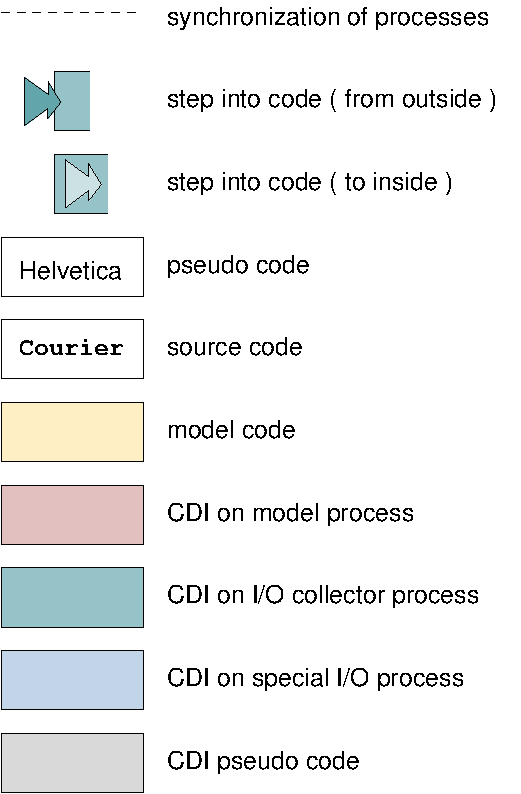
\includegraphics[scale=0.48]{../graphics/legend.pdf}}
\hspace{40pt}
\subfloat[Pseudo code encodeNBuffer]
{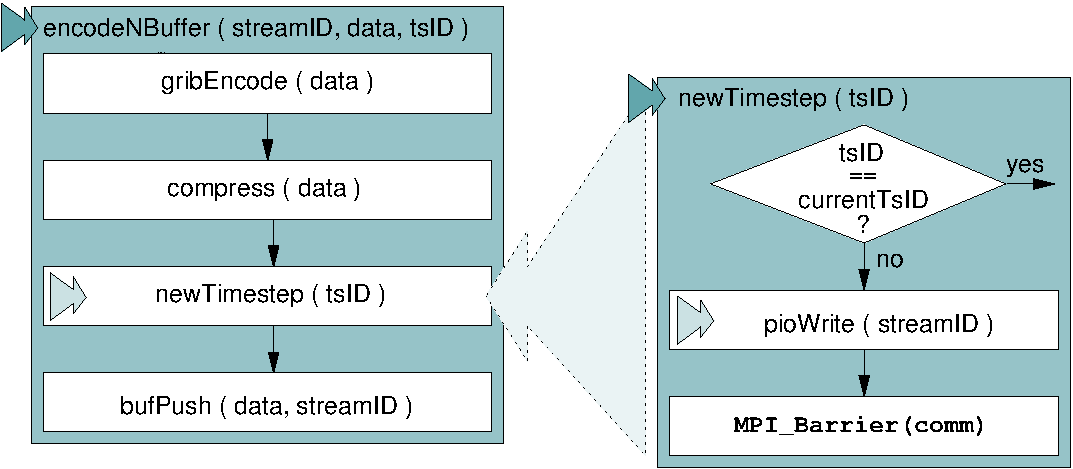
\includegraphics[scale=0.52]{../graphics/encodeNBuffer.pdf}}
%\vspace{-10pt}
\caption {Legend and pseudo code encodeNBuffer}
\index{legend}
\index{encodeNBuffer}
\label{legend}	
%\vspace{-10pt}
\end{figure}
On the I/O processes 
the excecution of the subprogram {\tt streamWriteVar} is controlled by the I/O 
 modes. To clearify the functioning we use pseudo code and
flowcharts as you can see in figure~\ref{legend}. 
The command 
\texttt{encodeNBuffer} abstracts the encoding, compressing and buffering
of the data for a variable. The data in a 
{\tt GRIB} file may not be mixed by time, so we need a command \texttt{newTimestep} 
to manage the flushing of the output buffers on the I/O server side. To 
achieve this, a \texttt{MPI\_Barrier} is used. 


\bigskip

I/O modes provided by {\pio}:

\bigskip

\hspace*{4mm}\begin{minipage}[]{15cm}
\begin{deflist}{\tt PIO\_FPGUARD\ } 
\item[{\htmlref{\tt PIO\_NONE}{PIONONE}}] 
one process collects, transposes, encodes, compresses, buffers and writes using 
{\tt C} {\tt fwrite}.
\item[{\htmlref{\tt PIO\_MPI}{PIOMPI}}] 
all processes collect, transpose, encode, compress, buffer and write using 
{\tt MPI\_File\_iwrite\_shared}.
\item[{\htmlref{\tt PIO\_ASYNCH}{PIOASYNCH}}]
one process writes the files using low level 
{\tt POSIX\_AIO}, the others collect, transpose, encode, compress and buffer.
\item[{\htmlref{\tt PIO\_FPGUARD}{PIOFPGUARD}}]
one process guards the fileoffsets, all others 
collect, transpose, encode, compress and write using {\tt C} {\tt fwrite}.
\item[{\htmlref{\tt PIO\_WRITER}{PIOWRITER}}]
one process writes the files using {\tt C} {\tt fwrite}, 
the others collect, transpose, encode, compress and buffer.
\end{deflist}
\end{minipage}


\section{{\tt PIO\_NONE}: $1$ process collects and writes using {\tt POSIX IO}}
\index{PIONONE@{\tt PIO\_NONE}}
\label{PIONONE}

The I/O mode {\tt PIO\_NONE} can only be run with one I/O process per physical 
node. This 
process collects, encodes, compresses, buffers and writes the data to the files 
attributed 
to his node. For low level file writing the {\tt C} standard \texttt{fwrite} 
is used. The advantages 
in comparison with the former serial writing are that the writing is done 
asynchronous with respect to the calculation and that the data is buffered. In 
addition it can be executed in parallel spread over physical nodes.

\begin{figure}[H]
\vspace{-10pt}
\centering
\subfloat[{\tt PIO\_NONE}]{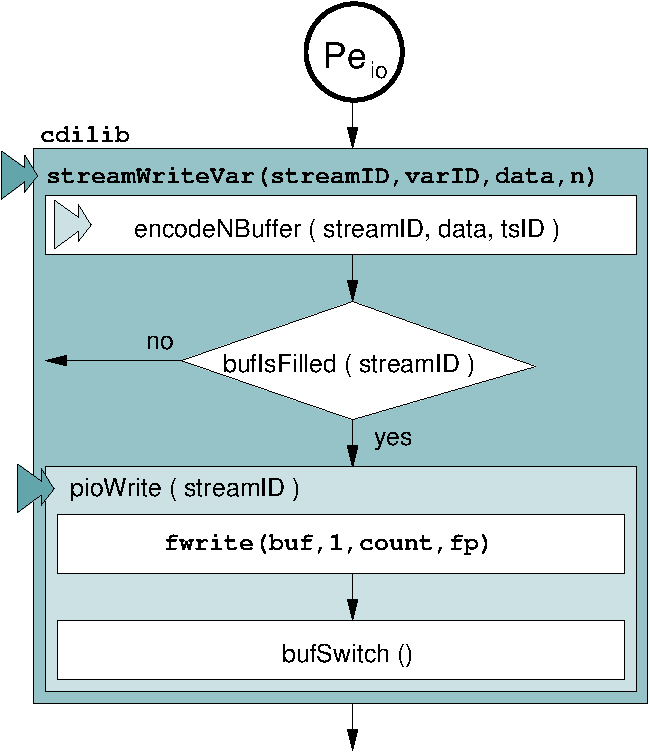
\includegraphics[scale=0.5]{../graphics/pio_none.pdf}}
\hspace{50pt}
\subfloat[{\tt PIO\_MPI}]{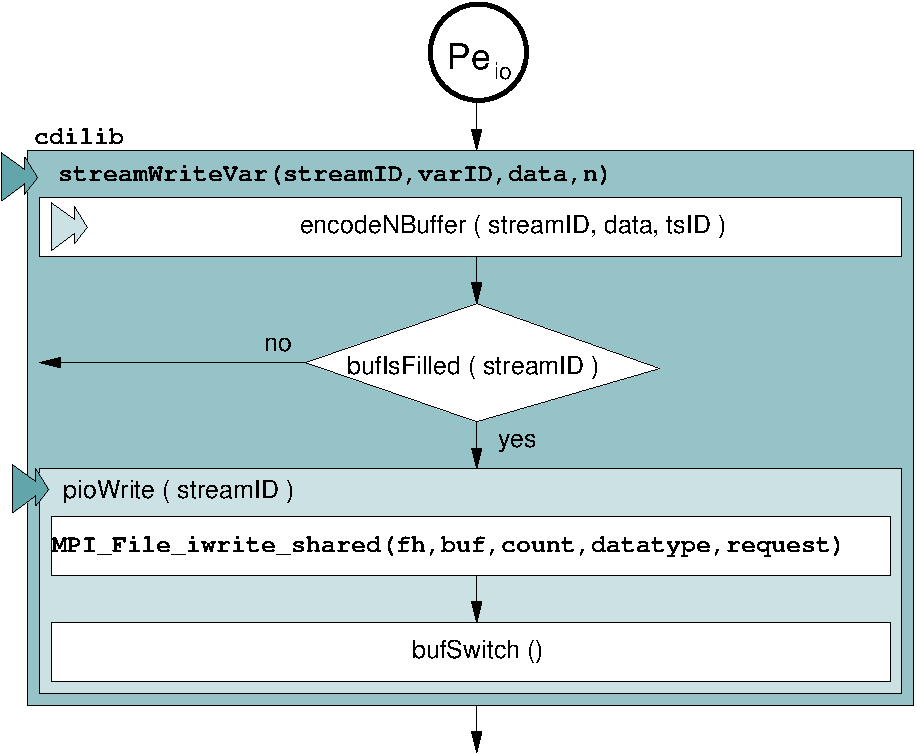
\includegraphics[scale=0.5]{../graphics/pio_mpi.pdf}}
\vspace{-10pt}
\caption {{\tt PIO\_NONE} and {\tt PIO\_MPI}}	
\vspace{-5pt}
\end{figure}

\section{{\tt PIO\_MPI}: $n$ processes collect and write using {\tt MPI IO}}
\index{PIOMPI@{\tt PIO\_MPI}}
\label{PIOMPI}

Data access using {\tt MPI} is the straight forward way to parallel file 
manipulation. With \\
{\tt MPI\_File\_iwrite\_shared} the processes have a shared 
file pointer available. The function is nonblocking and split collective. Like 
{\htmlref{\tt PIO\_NONE}{PIONONE}} the I/O mode {\tt PIO\_MPI} has no division 
of task within the I/O group, all processes collect, encode, compress, buffer and 
write to file. Writing in this I/O mode strongly depends on the {\tt MPI} 
implementation, the buffers used internally are of major importance for the 
performance of writing.

\section{{\tt PIO\_WRITER}: $n - 1$ processes collect and $1$ writes using 
{\tt POSIX IO}}
\index{PIOWRITER@{\tt PIO\_WRITER}}
\label{PIOWRITER}

\begin{figure}[H]
\vspace{-10pt}
\centering
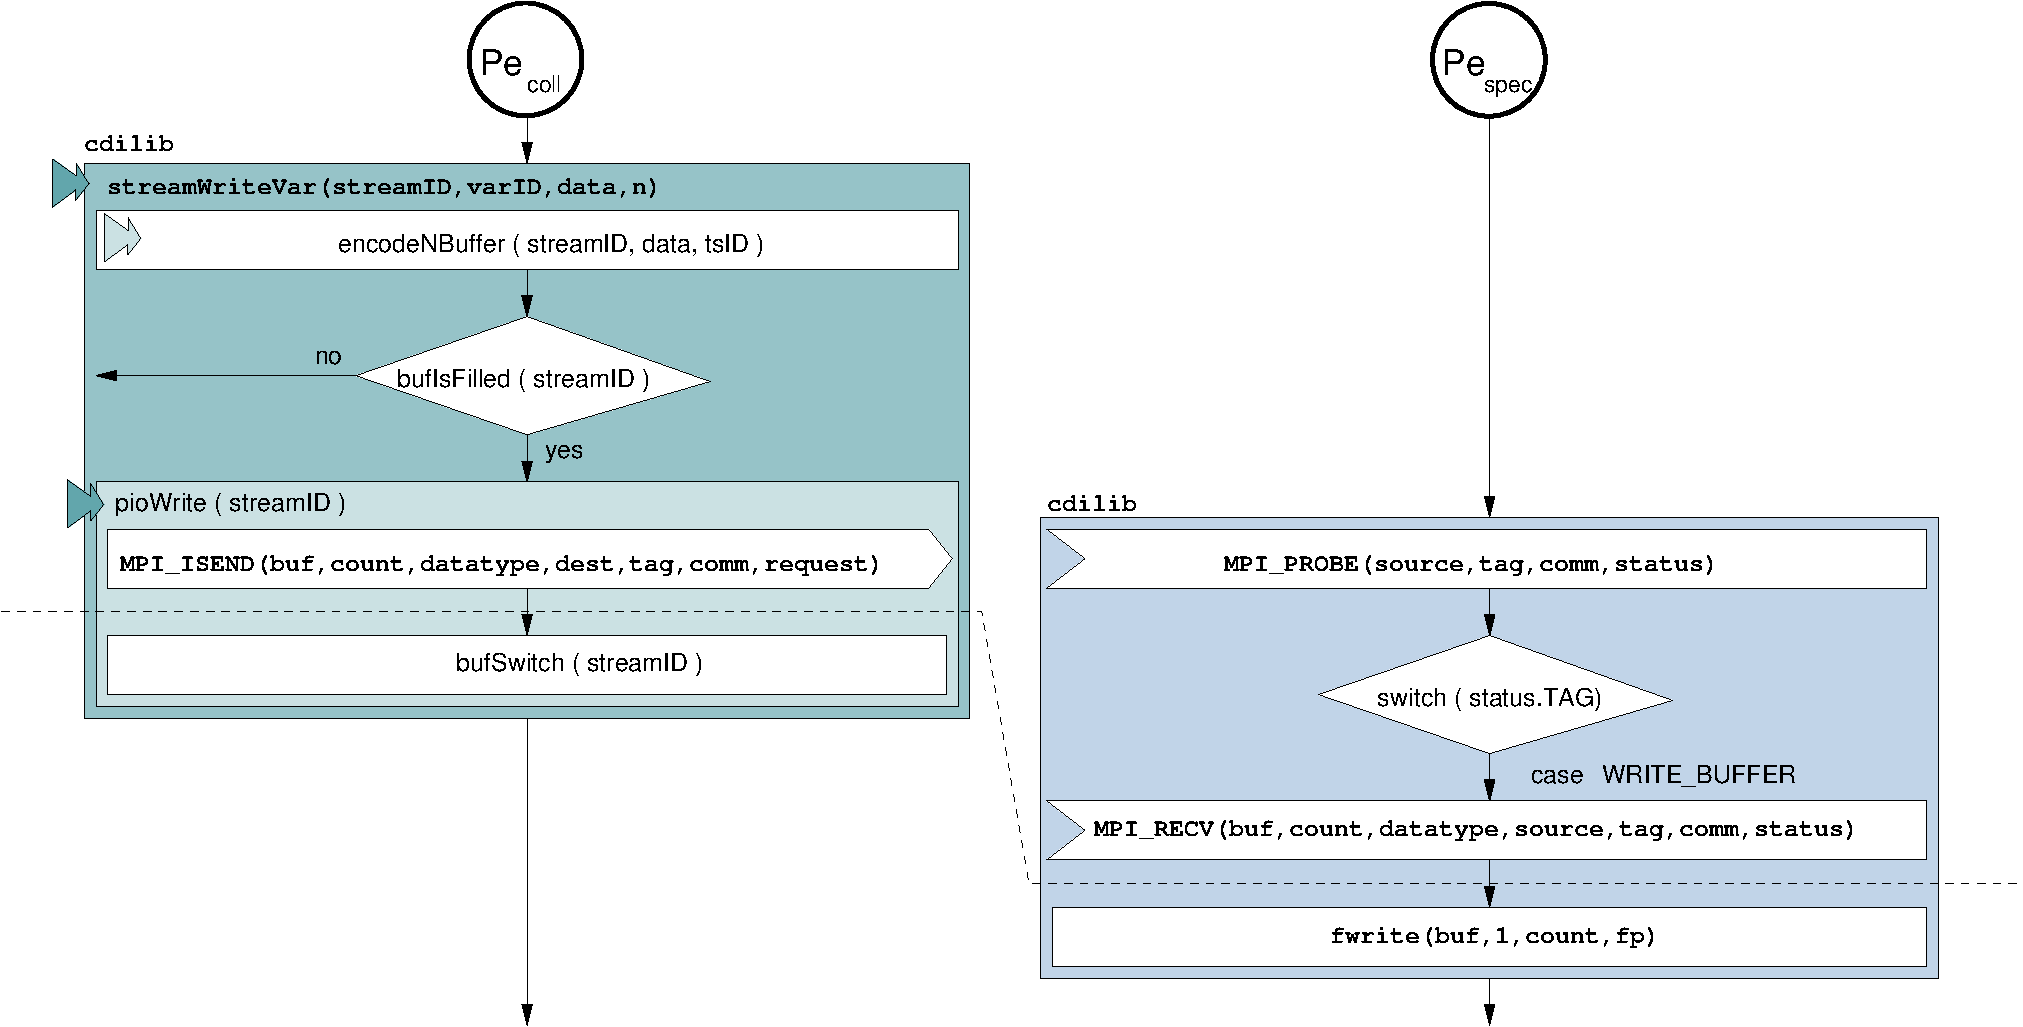
\includegraphics[scale=0.47]{../graphics/pio_writer.pdf}
\caption{{\tt PIO\_WRITER}}
\vspace{-10pt}
\end{figure}
If the I/O mode {\tt PIO\_WRITER} is chosen, the subtasks of writing are split
between the I/O processes. Just one process per physical node does the
low level writing  while the others collect, encode, compress and buffer 
the data. The writer is the process with the highest rank within the
I/O group on one physical node. Originating from {\htmlref{\tt pioInit}{pioInit}} 
he invokes a
backend server function, which he does not leave until he received messages from 
all  
collecting I/O processes to finalize.  A collector gets data from the calculating 
model processes via {\tt MPI RMA} communication, and, after encoding and
compressing it, pushes it to a double buffer. If the buffer is filled,
the contained data is send via \texttt{MPI\_Isend} to the writer, the 
collector
switches to the other buffer and continues his job. Before sending the
data he has to wait for a potentially outstanding
\texttt{MPI\_Request}. This might happen if the writer or the buffers
used by {\tt MPI} are overcommited and indicates that the ratio of
collectors and writers has to be checked. The writer is
polling using \texttt{MPI\_Probe} to look for incoming messages from
the collectors. One message per collecting process is tagged with the finalize 
command. All other messages contain a stream identifier, a buffer with
data to be written and a file manipulation instruction. There are three kinds of 
this commands:
1. open a file and write the data to it, 2. write the data to an
open file and 3. write the data to an open file and close it afterwards. 
For the file writing {\tt C} standard \texttt{fwrite} is used.

\section{{\tt PIO\_ASYNCH}: $n - 1$ processes collect and $1$ writes using 
{\tt POSIX AIO}} 
\index{PIOASYNCH@{\tt PIO\_ASYNCH}}
\label{PIOASYNCH}

The I/O mode {\tt PIO\_ASYNCH} is similar to {\tt PIO\_WRITER}, it only differs in
the method used for low level file writing. The asynchronous nonblocking I/O 
can be overlapped with processing, write orders are passed to the operating 
system. 

\section{{\tt PIO\_FPGUARD}: $n - 1$ processes collect and write using {\tt POSIX
 IO}}
\index{PIOFPGUARD@{\tt PIO\_FPGUARD}}
\label{PIOFPGUARD}

\begin{figure}[H]
\vspace{-10pt}
\centering
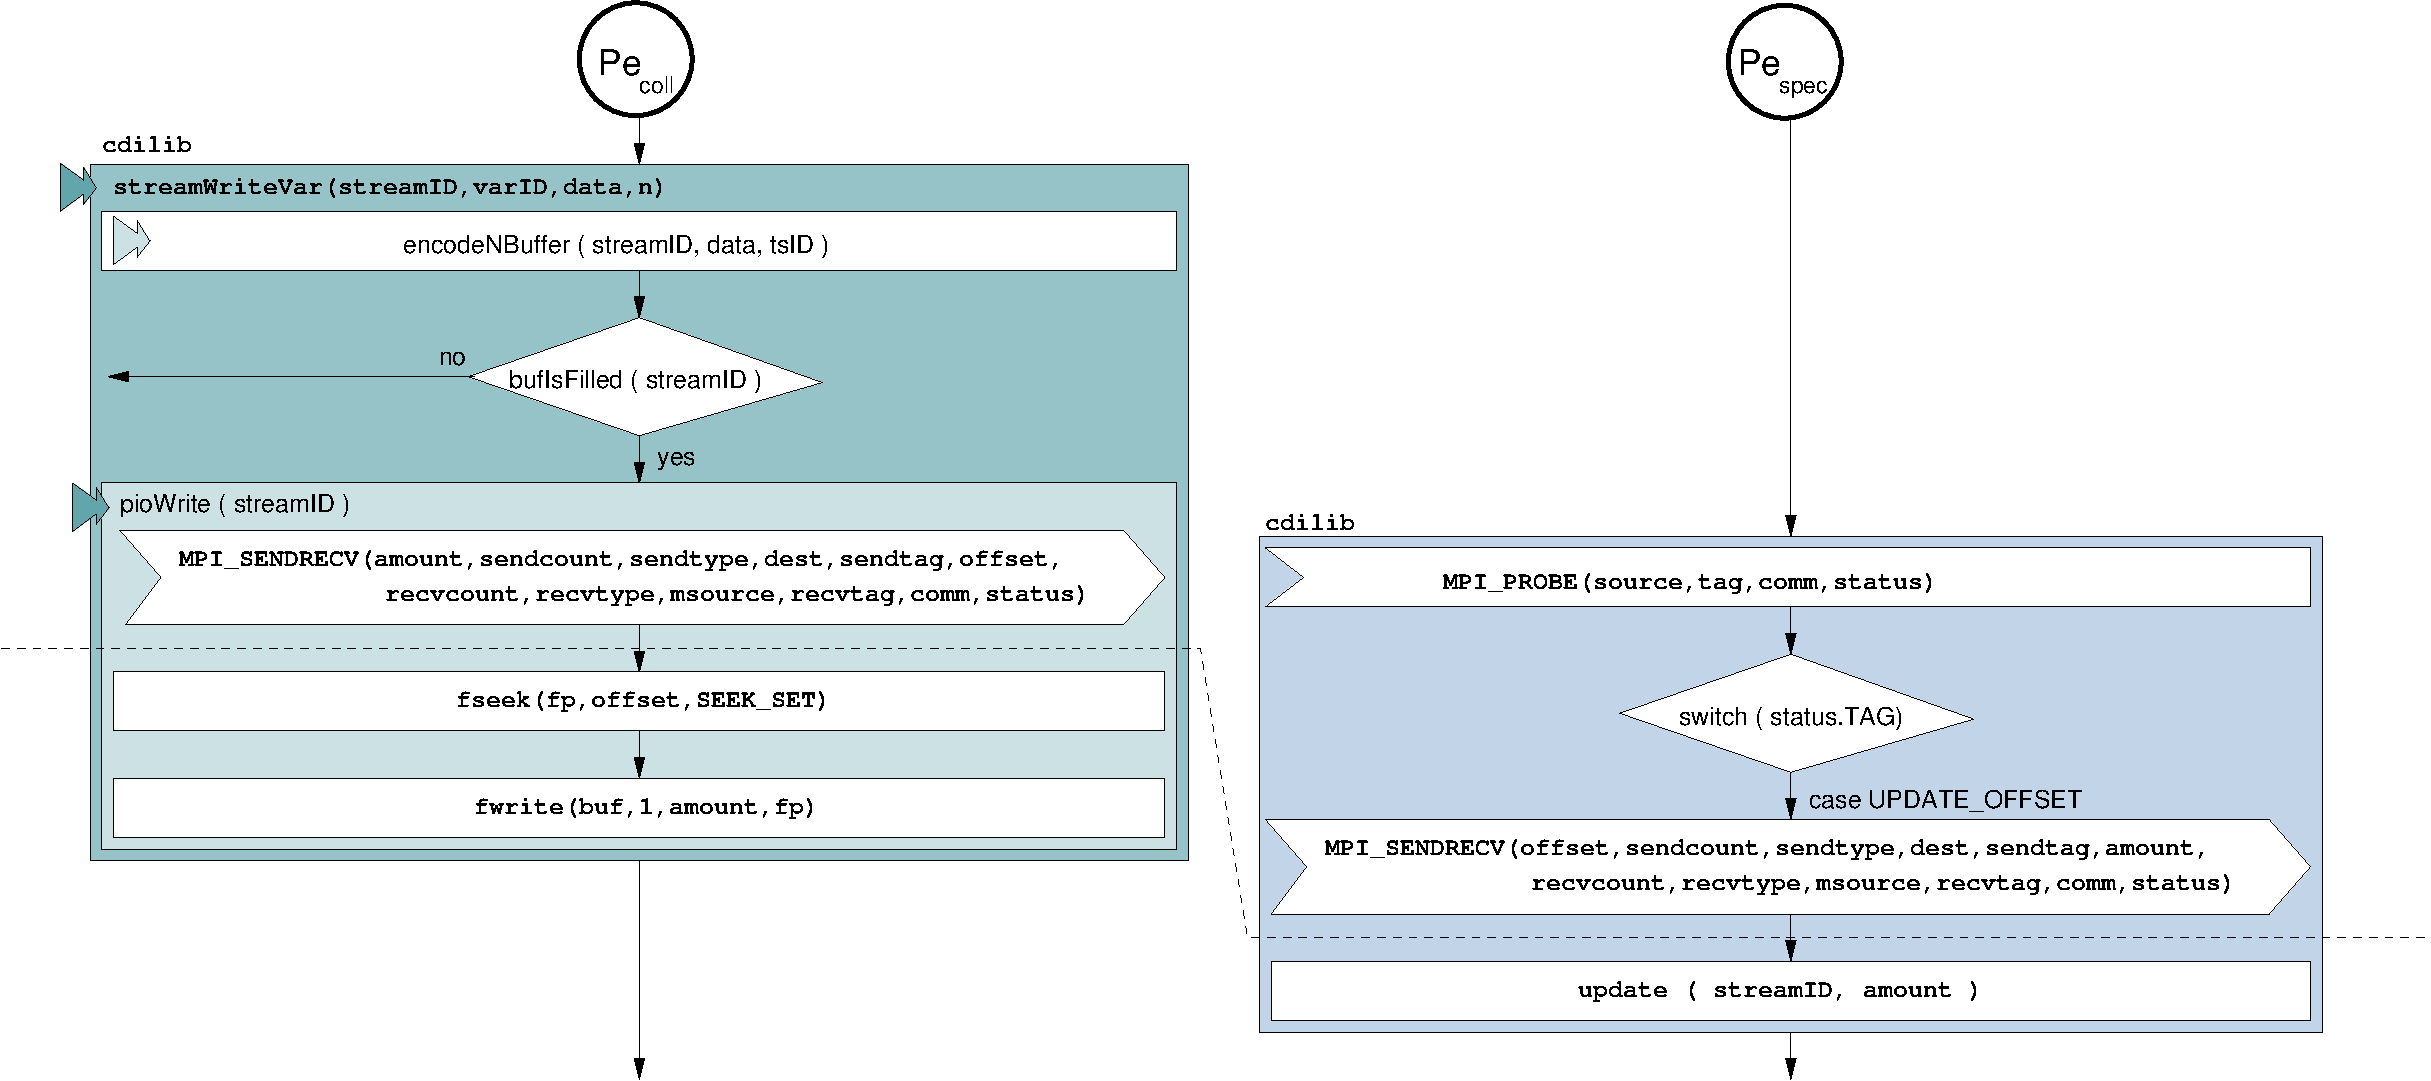
\includegraphics[scale=0.41]{../graphics/pio_fpguard.pdf}
\vspace{-10pt}
\caption{{\tt PIO\_FPGUARD}}
\vspace{-10pt}
\end{figure}
Writing a huge amount of data with a fixed file offset is a very fast
way of file writing. In this I/O mode one I/O process per physical 
node is spent to administrate the file offsets while the others do all the 
subtasks former defined for the parallel I/O. The functionality of this
collaboration is similar to
{\tt PIO\_WRITER}. Originating from {\htmlref{\tt pioInit}{pioInit}} the 
process with the highest rank calls a backend server 
function in which it is busy waiting 
for messages. The collecting I/O processes 
get data from the calculating model processes via {\tt MPI} RMA communication. 
The data is encoded, compressed and buffered. 
If the buffer is filled, the collector 
sends the count of the contained data to the ``file pointer guard'' and gets a 
file offset back. With the received offset the collector writes the data to 
file using {\tt C} standard
\texttt{fwrite} and goes on with his job. One message per collecting process 
is tagged with the finalize command. All other messages needed for 
the communication between the ``file pointer guard'' and the collectors 
contain a stream identifier, a numeric value holding the amount of buffered data
respectively the file offset and a command. There are three kinds of commands:
1. offset wanted for a file that will be newly opened, 2. offset wanted for an 
open file and 3. offset wanted for a file that will be closed after writing. 